\documentclass[10pt]{beamer}
\usetheme{metropolis}
% all imports
\usepackage{lmodern}
\usepackage[utf8]{inputenc}
\usepackage[T1]{fontenc}
\usepackage{appendixnumberbeamer}
\usepackage{hyperref}
\usepackage{booktabs}
\usepackage{bm}
\usepackage[scale=2]{ccicons}
\usepackage[outputdir=build]{minted}
\usepackage{pgfplots}
\usepackage{array,colortbl,xcolor}
\usepgfplotslibrary{dateplot}
\usepackage{setspace}
\usepackage{etoolbox}
\usepackage{xspace}
\usepackage{tikz}
\usetikzlibrary{shapes,arrows,positioning,fit,backgrounds}
\usepackage{tkz-euclide}

\AtBeginEnvironment{quote}{\singlespacing}


\AtBeginEnvironment{quote}{\singlespacing}

% new commands
\newcommand{\themename}{\textbf{\textsc{metropolis}}\xspace}
\newcommand{\vect}[1]{\bm{#1}}
\newcommand{\myprime}[1]{{#1}^{\prime}}
\newcommand{\grad}[2]{\nabla_{#1} {#2}}
\newcommand{\dotp}[2]{{#1}^{\top}{#2}}
\newcommand{\dotpPright}[2]{{#1}^{\top}\left({#2}\right)}
\newcommand{\outerp}[2]{\left({#1}\right){#2}^{\top}}
\newcommand{\Jacobian}[2]{\frac{\partial #1}{\partial #2}}
\newcommand{\Vocab}{\mathbb{V}}
\DeclareMathOperator*{\argmin}{arg\,min}

% Quote with author reference at the end
\let\oldquote\quote
\let\endoldquote\endquote
\renewenvironment{quote}[2][]
  {\if\relax\detokenize{#1}\relax
     \def\quoteauthor{#2}%
   \else
     \def\quoteauthor{#2~---~#1}%
   \fi
   \oldquote}
  {\par\nobreak\smallskip\hfill(\quoteauthor)%
   \endoldquote\addvspace{\bigskipamount}}



% definitions
\definecolor{blue}{RGB}{159, 192, 176}
\definecolor{green}{RGB}{160, 227, 127}
\definecolor{orange}{RGB}{243, 188, 125}
\definecolor{red}{RGB}{253, 123, 84}
\definecolor{nephritis}{RGB}{39, 174, 96}
\definecolor{emerald}{RGB}{46, 204, 113}
\definecolor{turquoise}{RGB}{39, 174, 96}
\definecolor{green-sea}{RGB}{22, 160, 133}
% Tikzstyles for Computation Graphs

% nodes
\tikzstyle{noop} = [circle, draw=none, fill=red, minimum size = 10pt]
\tikzstyle{op} = [circle, draw=red, line width=1.5pt, fill=red!70, text=black, text centered, font=\bf \normalsize, minimum size = 25pt]
\tikzstyle{op2} = [circle, draw=orange, line width=1.5pt, fill=orange!70, text=black, text centered, font=\bf \normalsize, minimum size = 25pt]
\tikzstyle{op3} = [circle, draw=orange, line width=1.5pt, fill=orange!70, text=black, text centered, font=\bf \scriptsize, minimum size = 7pt]
\tikzstyle{placeholder} = [circle, draw=red, line width=1.5pt, fill=red!30, text=black, text centered, font=\bf  \normalsize, minimum size = 25pt]
\tikzstyle{state} = [circle, draw=blue, line width=1.5pt, fill=blue!70, text=black, text centered, font=\bf \normalsize, minimum size = 25pt]
\tikzstyle{gradient} = [circle, draw=nephritis, line width=1.5pt, fill=nephritis!60, text=black, text centered, font=\bf \normalsize, minimum size = 25pt]
\tikzstyle{gradient2} = [circle, draw=green2, line width=1.5pt, fill=green2!60, text=black, text centered, font=\bf \normalsize, minimum size = 25pt]
\tikzstyle{textonly} = [draw=none, fill=none, text centered, font=\bf \normalsize]

% edges
% \tikzstyle{tedge}  = [draw, thick, >=stealth, ->]
\tikzstyle{tedge}  = [draw, thick, >=latex, ->]
\tikzstyle{tedge_dashed}  = [draw, thick, >=latex, ->, dashed]

% namedscope
\tikzstyle{namedscope} = [circle, draw=orange, line width=1.5pt, fill=orange!60, align=center, inner sep=0pt]

% \tikzstyle{container} = [draw=none, rectangle, dotted, inner ysep=1.5em]
% \tikzstyle{novertex} = [draw=none, fill=none, text centered]
% \tikzstyle{predicate} = [ellipse, draw, thick, text centered, rounded corners, minimum size=30pt]
% \tikzstyle{aux} = [rectangle, draw, thick, text centered, rounded corners, minimum size=30pt]
% \tikzstyle{ledge}  = [draw, dashed, thick, >=stealth, ->]
% \tikzstyle{pedge}  = [draw, thick, >=stealth, ->]



\title{Anytime Dynamic A*: \\
\Large An Anytime Replanning Algorithm} 
\date{\today}
\author{Autores: Maxim Likhachev, Dave Ferguson, Geoff Gordon, Anthony Stentz e Sebastian Thrun\\
\\Paula Moraes}
\institute{\textbf{IME-USP}: Instituto de Matemática e Estatística - Universidade de São Paulo}

\titlegraphic{
            \hspace{9cm}
            
\includegraphics[scale=0.2]{images/liamflogo.png}
}



\begin{document}
\nocite{Sutton98a}

\maketitle



\begin{frame}{Artificial Intelligence}

\begin{figure}[h]
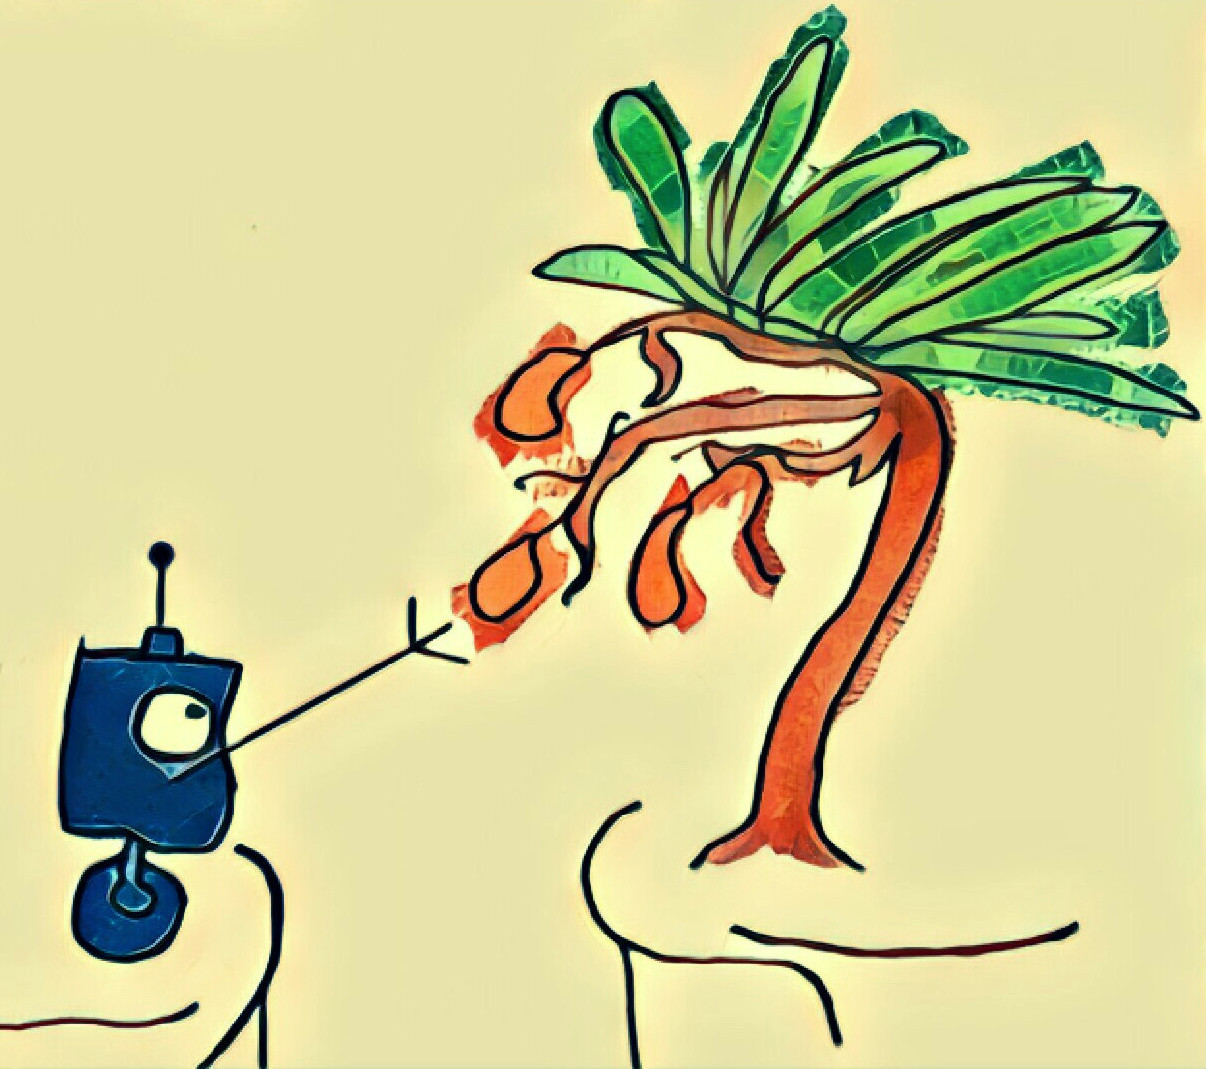
\includegraphics[width=5cm]{images/robo.jpg}
\end{figure}
\end{frame}


\begin{frame}{Reinforcement Learning schema}
\begin{figure}[ht!]
\centering

\scalebox{1.12}{
\begin{tikzpicture}[auto]

% nodes =============================
\node  (agent) {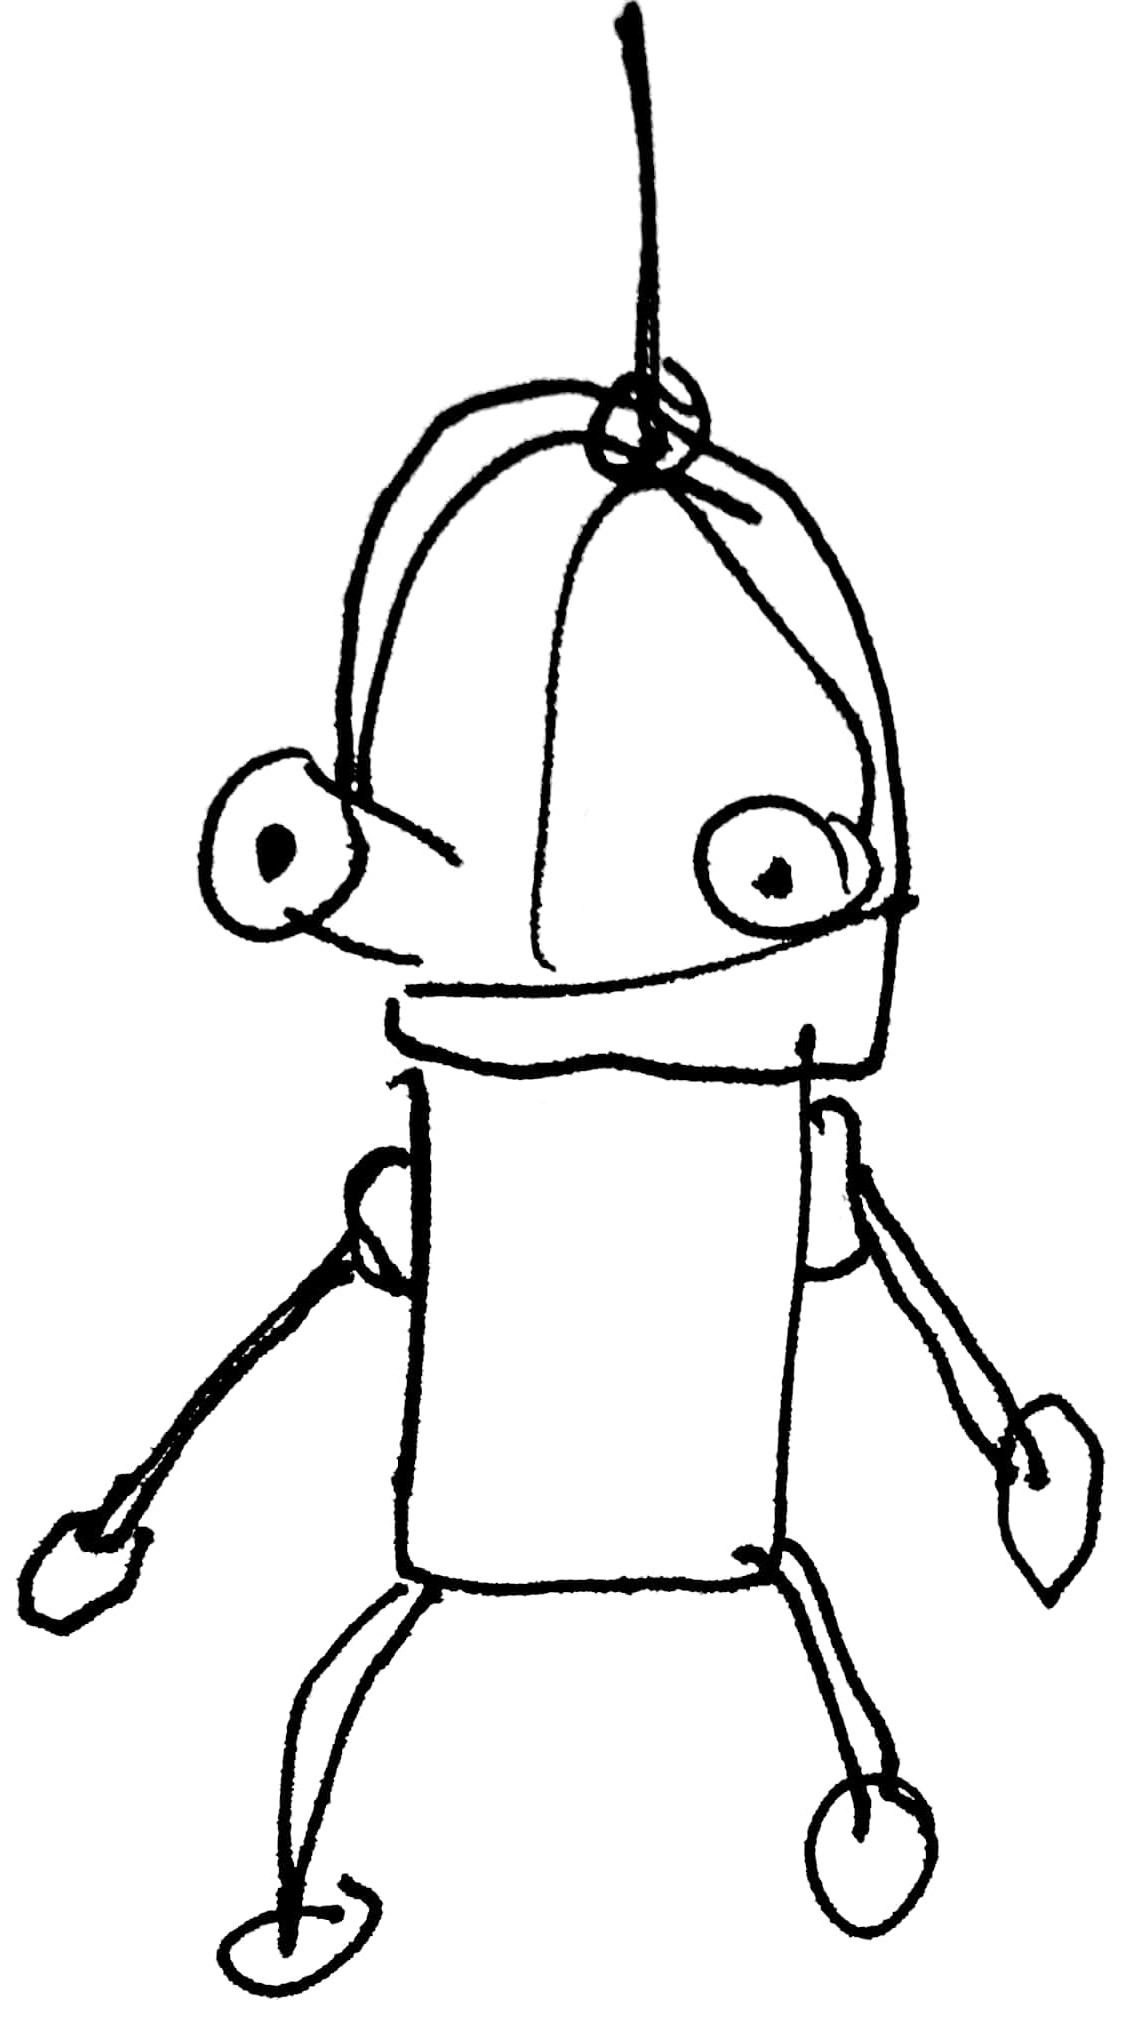
\includegraphics[width=.15\textwidth]{images/agent.jpg}};
\node[state, right=70pt of agent] (env) {\Large{Environment}};
\node[textonly, above left=4.5pt and -30.0pt of env] (inv1) {};
\node[textonly, above right=0.5pt and -30.5pt of agent] (inv2) {};
\node[textonly, below left=4.5pt and -30.0pt of env] (inv3) {};
\node[textonly, below right=0.5pt and -30.5pt of agent] (inv4) {};
\node[textonly, below=-3.8pt of agent] (label) {Agent};



% edges =============================

\path[tedge, nephritis!60, line width=1mm] (inv2) edge [out=80,in=120] node[above right] {action} (inv1);
\path[tedge, nephritis!60, line width=1mm] (inv3) edge [out=-120,in=-80] node[below right] {state} (inv4);
\path[tedge, nephritis!60, line width=1mm] (env) edge node[above] {reward} (agent);

\end{tikzpicture}
} % scalebox
\end{figure}

\end{frame}

\begin{frame}[fragile]{Q-learning}
\begin{figure}[ht!]
\centering
\scalebox{0.78}{
\begin{tikzpicture}
% 3x3 grid 
\draw[opacity=0.4] (0,0) rectangle (3,3);
\draw[draw=black,thick] (0,0) grid (3,3);
\node (00) at (0.5,2.5) {\Large -1};
\node (01) at (1.5,2.5) {\Large -1};
\node (02) at (2.5,2.5) {\Large -1};
\node (10) at (0.5,1.5) {\Large -1};
\node (11) at (1.5,1.5) {\Large -8};
\node (12) at (2.5,1.5) {\Large -1};
\node (20) at (0.5,0.5) {\Large -1};
\node (21) at (1.5,0.5) {\Large -8};
\node (22) at (2.5,0.5) {\Large 10};


\node[textonly, left=60pt of 20] (inv1) {};
\node[textonly, left=2pt of 20] (inv2) {};

\node[boxtextonly, below=10pt of 21] (label1) {states and\\rewards};
\path[tedge, nephritis!60, line width=1mm] (inv1) -- (inv2);

% 3x3 actions 
\node[textonly, right=50pt of 12] (inv3) {};
\node[textonly, right=30pt of inv3] (inv4) {};
\node[textonly, left=30pt of inv3] (inv5) {};
\node[textonly, above=30pt of inv3] (inv6) {};
\node[textonly, below=30pt of inv3] (inv7) {};
\node[textonly, right=45pt of label1] (label2) {actions};
\path[tedge, orange!120, line width=1mm] (inv3) -- (inv4);
\path[tedge, orange!120, line width=1mm] (inv3) -- (inv5);
\path[tedge, orange!120, line width=1mm] (inv3) -- (inv6);
\path[tedge, orange!120, line width=1mm] (inv3) -- (inv7);

% Q table
\node[textonly, right=5pt of inv4] (table) {$\begin{bmatrix}Q(1,\uparrow) & Q(1,\downarrow) & Q(1,\leftarrow) & Q(1,\rightarrow) \\ \vdots & \vdots & \vdots & \vdots \\Q(9,\uparrow) & Q(9,\downarrow) & Q(9,\leftarrow) & Q(9,\rightarrow)\end{bmatrix}$};
\node[textonly, right=80pt of label2] (label3) {Q-table};


 \end{tikzpicture}
} % scalebox
\end{figure}

\end{frame}

\begin{frame}[fragile]{RL and feature engineering}
\begin{figure}[ht!]
\centering

\scalebox{0.65}{
\begin{tikzpicture}[auto]

% operations =============================

\begin{scope}[xshift=0cm,yshift=0cm]
            \begin{scope}[xshift=0cm,yshift=0cm]
            \node (x1) at (2,1.5) {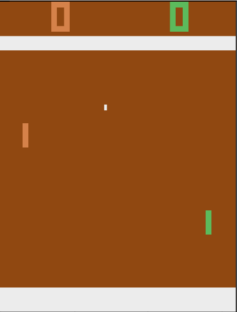
\includegraphics[width=.25\textwidth]{images/frame1.png}};
            \end{scope}
            \begin{scope}[xshift=-0.6cm,yshift=-0.6cm]
            \node (x2)  at (2,1.5) {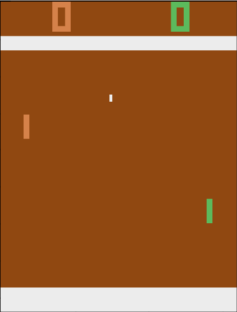
\includegraphics[width=.25\textwidth]{images/frame2.png}};
            \end{scope}
            \begin{scope}[xshift=-1.2cm,yshift=-1.2cm]
            \node (x3)  at (2,1.5) {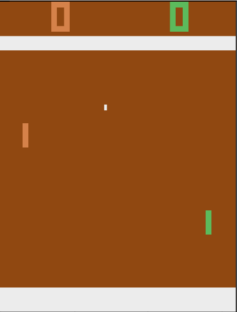
\includegraphics[width=.25\textwidth]{images/frame1.png}};
            \end{scope}  
\end{scope}

\node[op] (h2)  at (7,1) {{\LARGE$\begin{bmatrix}1.8\\1.7\\1.6\end{bmatrix}$}};

\node[textonly, right=10pt of h2] (inv1) {};
\node[op, right=60pt of h2] (f) {{\LARGE$f$}};
\node[textonly, right=2pt of f] (inv2) {};

\node[textonly, right=8pt of x2] (inv3) {};
\node[textonly, right=55pt of inv3] (inv4) {};


\node[textonly, right=30pt of inv2] (result) {{\LARGE$\begin{bmatrix}Q(s,a_1)\\ \vdots \\Q(s,a_n)\end{bmatrix}$}};



%edges
\path[tedge, orange!120, line width=1.5mm]  (inv1) -- (f);
\path[tedge, orange!120, line width=1.5mm]  (inv2) -- (result);
\path[tedge, orange!120, line width=1.5mm]  (inv3) -- (inv4);

 %info
 
 \node[textonly, above=85pt of h2] (inv5) {\LARGE{The pong game can have $256^{84\times84\times3}$ different states.}};

\end{tikzpicture}
} % scalebox
\end{figure}

\end{frame}

\begin{frame}[fragile]{Deep Q-learning}
\begin{figure}[ht!]
\centering

\scalebox{0.8}{
\begin{tikzpicture}[auto]

% operations =============================

\begin{scope}[xshift=0cm,yshift=0cm]
            \begin{scope}[xshift=0cm,yshift=0cm]
            \node (x1) at (1,1) {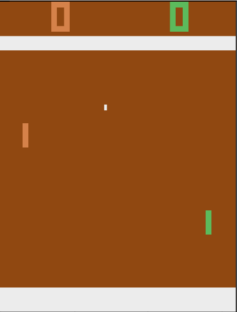
\includegraphics[width=.35\textwidth]{images/frame1.png}};
            \end{scope}
            \begin{scope}[xshift=-0.6cm,yshift=-0.6cm]
            \node (x2)  at (1,1) {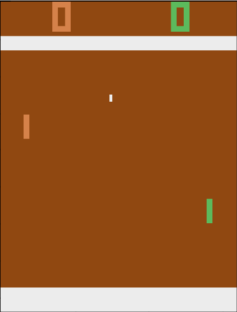
\includegraphics[width=.35\textwidth]{images/frame2.png}};
            \end{scope}
            \begin{scope}[xshift=-1.2cm,yshift=-1.2cm]
            \node (x3)  at (1,1) {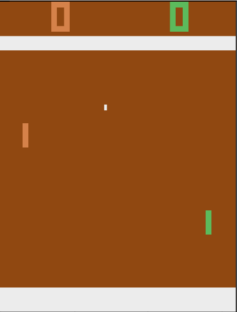
\includegraphics[width=.35\textwidth]{images/frame1.png}};
            \end{scope}  
\end{scope}


\node[textonly, right=10pt of x2] (inv1) {};
\node[op, right=60pt of x2] (f) {{\LARGE$f$}};
\node[textonly, right=2pt of f] (inv2) {};
\node[textonly, right=30pt of inv2] (result) {{\LARGE$\begin{bmatrix}Q(s,a_1)\\ \vdots \\Q(s,a_n)\end{bmatrix}$}};



%edges
\path[tedge, orange!120, line width=1.5mm]  (inv1) -- (f);
\path[tedge, orange!120, line width=1.5mm]  (inv2) -- (result);

\end{tikzpicture}
} % scalebox
\end{figure}
\end{frame}

\begin{frame}[fragile]{Deep Q-learning}
\begin{figure}[ht!]
\centering

\scalebox{0.8}{
\begin{tikzpicture}[auto]

% operations =============================

\begin{scope}[xshift=0cm,yshift=0cm]
            \begin{scope}[xshift=0cm,yshift=0cm]
            \node (x1) at (1,1) {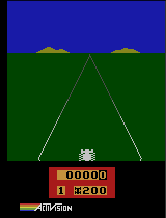
\includegraphics[width=.35\textwidth]{images/enduro.png}};
            \end{scope}
            \begin{scope}[xshift=-0.6cm,yshift=-0.6cm]
            \node (x2)  at (1,1) {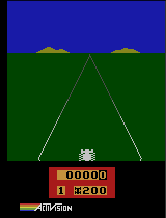
\includegraphics[width=.35\textwidth]{images/enduro.png}};
            \end{scope}
            \begin{scope}[xshift=-1.2cm,yshift=-1.2cm]
            \node (x3)  at (1,1) {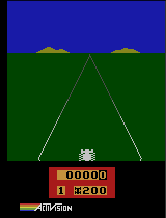
\includegraphics[width=.35\textwidth]{images/enduro.png}};
            \end{scope}  
\end{scope}


\node[textonly, right=10pt of x2] (inv1) {};
\node[op, right=60pt of x2] (f) {{\LARGE$f$}};
\node[textonly, right=2pt of f] (inv2) {};
\node[textonly, right=30pt of inv2] (result) {{\LARGE$\begin{bmatrix}Q(s,a_1)\\ \vdots \\Q(s,a_n)\end{bmatrix}$}};



%edges
\path[tedge, orange!120, line width=1.5mm]  (inv1) -- (f);
\path[tedge, orange!120, line width=1.5mm]  (inv2) -- (result);

\end{tikzpicture}
} % scalebox
\end{figure}
\end{frame}


\begin{frame}[allowframebreaks]{Referências}

  \bibliography{my_references}
  \bibliographystyle{abbrv}

\end{frame}




\end{document}